\chapter{State of the Art v oblasti HPC-as-a-Service}
Superpočítače a jejich výkon byl v minulosti vyhrazen pouze pro oblast výzkumu a vývoje. HPC infrastruktura byla k dispozici vládním, lékařským a výzkumným organizacím nebo inovativním filmařům. K majoritním případům užití superpočítačů v této době patřily simulace jaderných testů, mapování lidského genomu nebo „oživování dinosaurů“ ve filmech.

V současné době však dochází k masivnímu vzestupu datově náročných technologií. Typickým příkladem může být problematika umělé inteligence nebo problémy vyžadující masivní paralelismus\footnote{Masivní paralelismus je technika využívající velkého počtu procesorů či samotných počítačů k paralelnímu zpracování úloh.}. Tento fakt nutí širší okruh organizací zkoumat problematiku vysoce výkonného počítání. Ne každá společnost však má čas, peníze a odborné znalosti potřebné k jejich nasazení.

Z toho důvodu mohou tyto společnosti namísto náročného sestavování a správ superpočítačových clusterů využít již hotová řešení HPC jako služby (HPC-as-a-Service/HaaS). Díky HPC poskytovanému jako služba mohou organizace v některých případech spolupracovat s dodavatelem na konfiguraci infrastruktury, kterou potřebují pro své konkrétní výpočetní potřeby. Namísto nákupu nebo pronájmu hardwaru či softwaru si je však předplatí prostřednictvím modelu spotřeby „Pay for what you consume“ \cite{Rand20201203}.

\section{Výhody HPC-as-a-Service}
HPC poskytované jako služba má výhody oproti hostování vlastní HPC infrastruktury. První důležitou výhodou může být model spotřeby „Pay for what you consume“, který byl již zmiňován výše. Zákazník tak platí jen za zdroje, které skutečně využil. Vlastní řešení, konstrukce a následná správa vysoce výkonných výpočetních clusterů je velmi náročná na zdroje.

Společnosti či organizace poskytující HPC-as-a-Service mají tendenci rychleji integrovat novější technologie. Tyto technologie jsou pak přístupné uživatelům využívající jejich služeb. Někteří poskytovatelé HaaS umožňují jejich zákazníkům provádění aktualizací či škálování\footnote{Škálování je pojem vyjadřující navyšování kapacit.} výpočetních kapacit na vyžádání. \cite{Wiggers20220120}

\section{Případy užití}
V dnešní době se poskytovatelé HPC-as-a-Service snaží co nejvíce přizpůsobit požadavkům jejich zákazníků. HaaS využívají společnosti, které pro řešení jejich problémů vyžadují vysoce výkonné či paralelní zpracování dat. Poměrně velký segment zákazníků tvoří oblast Automotive\footnote{Segment automobilového průmyslu.}, ti využívají HPC například ke zkrácení času simulací proudění tekutin či plynů. Při využití výpočetních clusterů nejen oboru Automotive dochází k přesnějším a rychleji dosaženým výsledkům při vývoji. Dalším oborem, ve kterém je HPC hojně využíváno, je obor lékařství. Vývoj léčiv je díky paralelnímu zpracovaní dat na superpočítačích efektivnější a rychlejší, dochází pak i k minimalizaci vzniku chyb.

HPC je využíváno v mnoha dalších oborech či odvětvích, patří tam i obor výzkumu a vývoje. HPC umožňuje analyzovat rozsáhlé datové soubory v poměrně krátkém čase a sdílet výsledky se spolupracovníky. Dále je HPC využíváno třeba ke 3D modelování a renderování scén, toho využívají grafická, herní a filmová studia.

Obrázek \ref{fig:haas} ilustruje využití HPC-as-a-Service / HaaS.

\begin{figure}[!h]
	\centering
	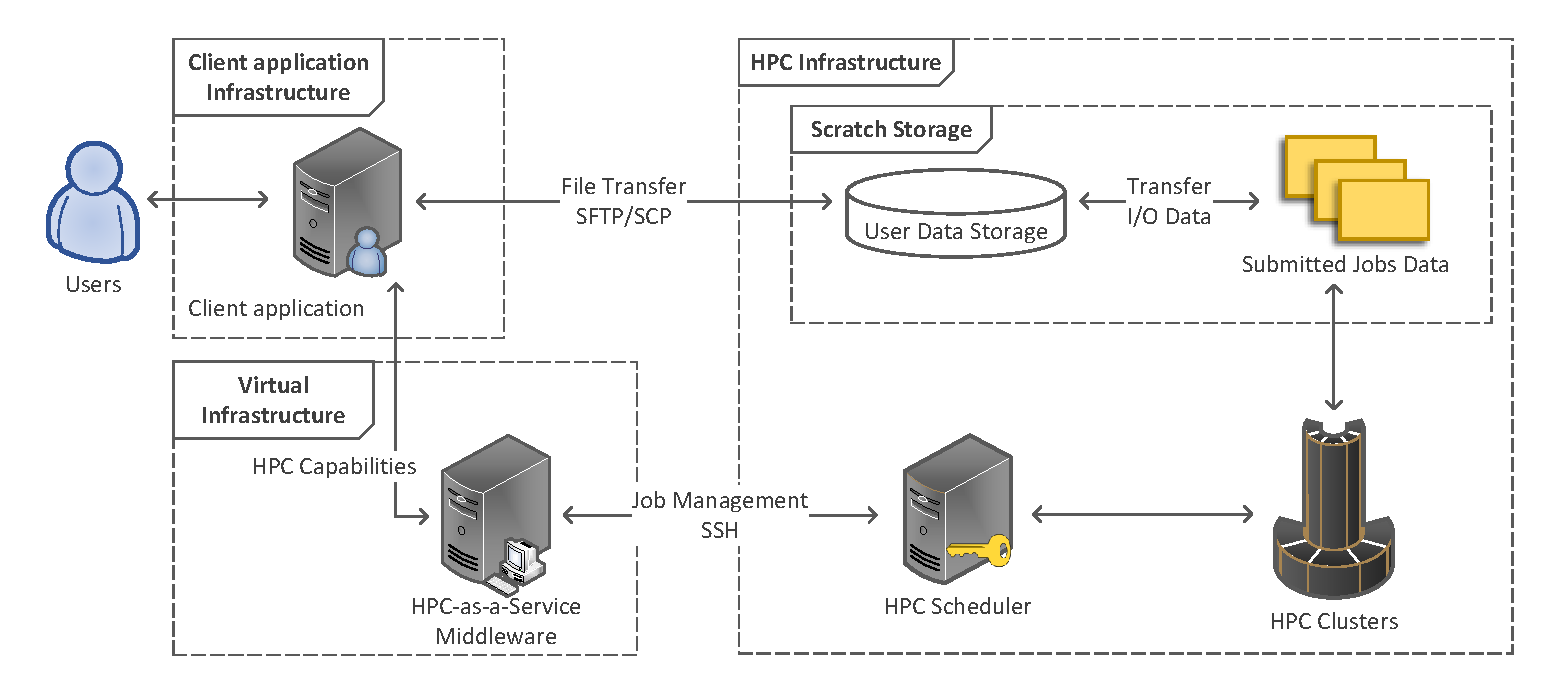
\includegraphics[width=1\textwidth]{Figures/haas.pdf}
	\caption{HPC-as-a-Service / HaaS \cite{uG7wIvjQiIli6kO9}}
	\label{fig:haas}
\end{figure}

\section{Největší poskytovatelé platforem HaaS}
Mezi největší poskytovatele HPC-as-a-Service v době psaní této práce patří společnosti Hewlett Packard Enterprise\footnote{\href{https://www.hpe.com/us/en/compute/hpc.html}{https://www.hpe.com/us/en/compute/hpc.html}}(HPE) a Atos\footnote{\href{https://atos.net/en/}{https://atos.net/en/}}. Obě tyto společnosti se dlouhodobě specializují na poskytování IT služeb.

\subsection{HPE Greenlake}
HPE nabízí z pohledu HaaS řešení, které bylo pojmenováno jako HPE Greenlake\footnote{\href{https://www.hpe.com/us/en/greenlake/high-performance-compute.html}{https://www.hpe.com/us/en/greenlake/high-performance-compute.html}}. Pro potřeby zákazníků poskytuje platforma HPE GreenLake jednoduché a bezpečné řešení návrhu či využívání vlastní vzdálené HPC infrastruktury bez nutnosti správy fyzických výpočetních clusterů. Mezi hlavní výhody této služby patří obchodní model „Pay for what you consume“. Využívání HPC zdrojů je měřeno a zákazník platí jen za to, co skutečně spotřeboval. Protože požadavky na pracovní zátěž HPC mohou kolísat, platforma HPE Greenlake umožňuje měnit konfigurace HPC kapacit. Výpočetní clustery, které jsou součástí infrastruktury zmiňované služby, jsou pravidelně aktualizovány po stránce hardwaru i softwaru. Uživateli to přináší nové možnosti bez nutnosti jakéhokoli zásahu. Na obrázku \ref{fig:greenlake} se nachází snímek z aplikace sloužící ke konfiguraci, správě a sledování využití výpočetních kapacit služby HPE Greenlake \cite{IN09sfzqoa3sLbg4}.

\begin{figure}[!h]
	\centering
	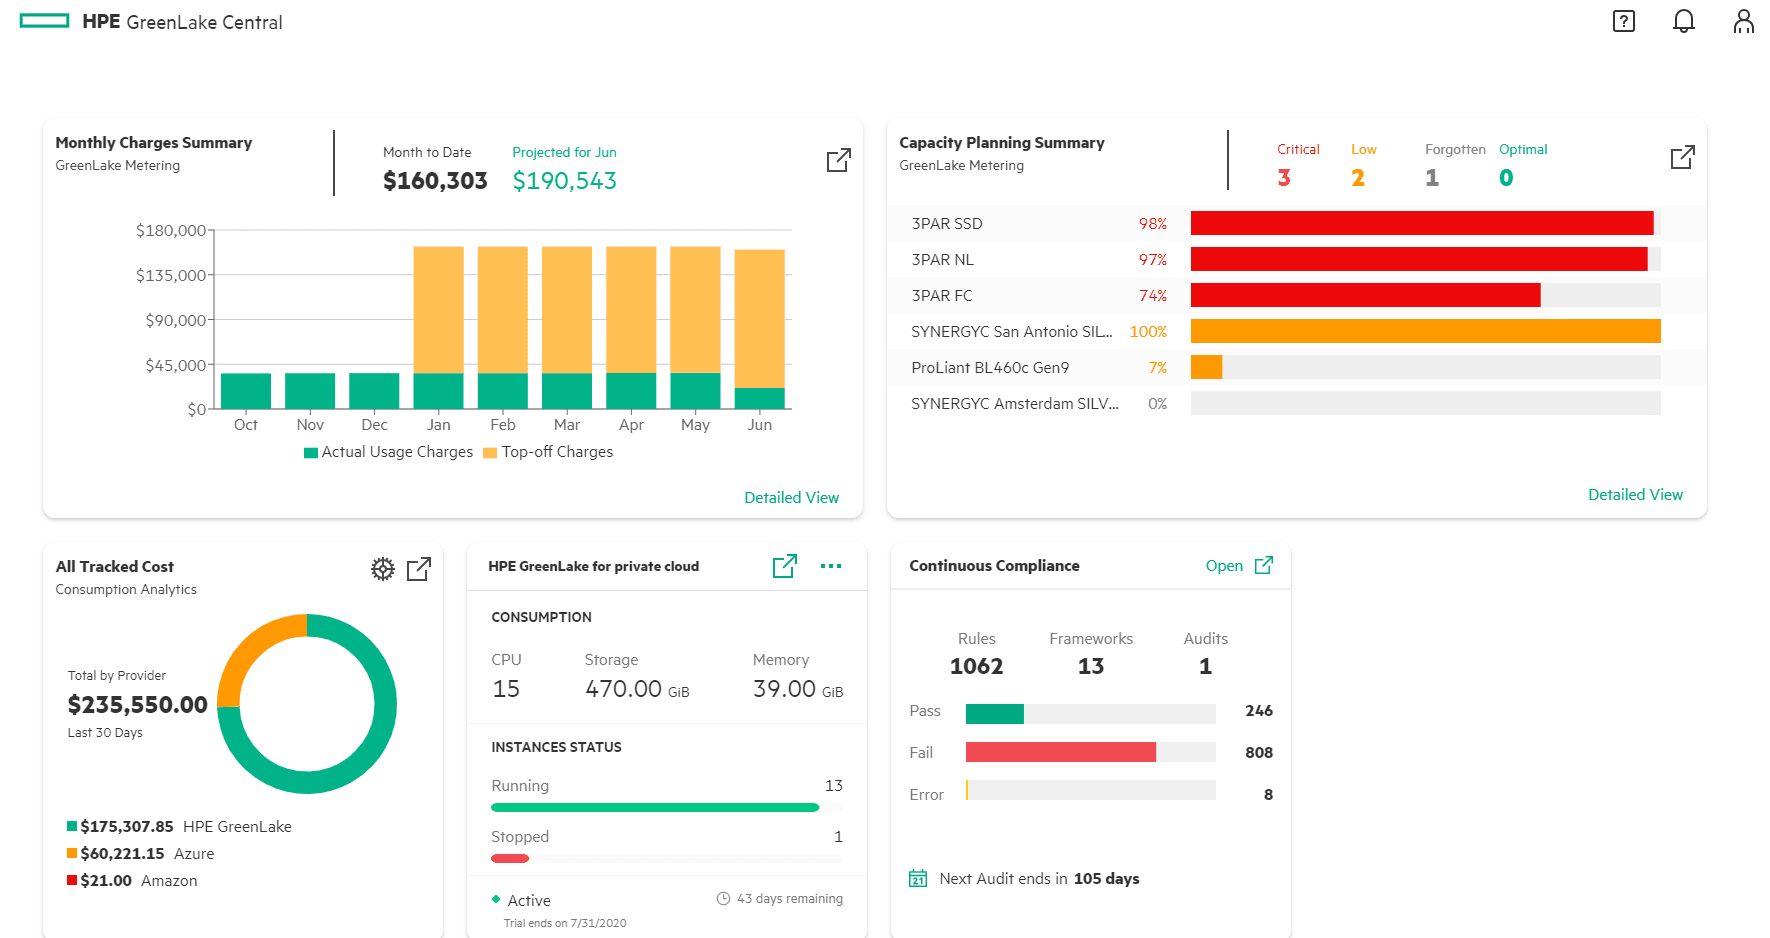
\includegraphics[width=1\textwidth]{Figures/hpe-greenlake-central.png}
	\caption{Snímek aplikace HPE Greenlake Central \cite{Showalter20200616}}
	\label{fig:greenlake}
\end{figure}
\newpage

\subsection{Nimbix JARVICE XE}
Společnost Atos nabízí své vlastní řešení problematiky HPC-as-a-Service v podobě platformy JARVICE™ XE\footnote{\href{https://www.nimbix.net/jarvicexe}{https://www.nimbix.net/jarvicexe}}. Tato platforma umožňuje správu libovolné HPC úlohy na libovolném HPC clusteru. Nezáleží na tom, zda se výpočetní cluster nachází v soukromém datacentru uživatele nebo v cloudu. JARVICE™ XE poskytuje akcelerované aplikace a pracovní postupy, které využívají různorodou infrastrukturu. Podpora je zajištěna například i pro platformu InfiniBand\footnote{\href{https://www.nvidia.com/en-us/networking/products/infiniband/}{https://www.nvidia.com/en-us/networking/products/infiniband/}} a výpočetní jednotky pro paralelní zpracování dat. Společnost navíc uživatelům platformy umožňuje snadno přejít z lokálních řešení na veřejné cloudové systémy nebo spravovat interní systémy jako soukromé cloudy. 

Správa HPC aplikací prostřednictvím zmiňované platformy probíhá přes rozhraní zvané The Smart HPC Web Portal. Toto rozhraní uživatelům systému zaručuje bezpečný a přímý přístup ke všem prostředkům a aplikacím. Po přihlášení má uživatel přístup ke kompletnímu pracovnímu prostředí přizpůsobenému jeho pracovní roli. Odtud může načítat a spravovat data, nastavovat parametry simulací, spouštět výpočty, sledovat jejich průběh a poté přejít k následnému zpracování a vizualizaci výsledků. Na obrázku \ref{fig:atos-dashboard} se nachází snímek obrazovky popisované aplikace.





\begin{figure}[!h]
	\centering
	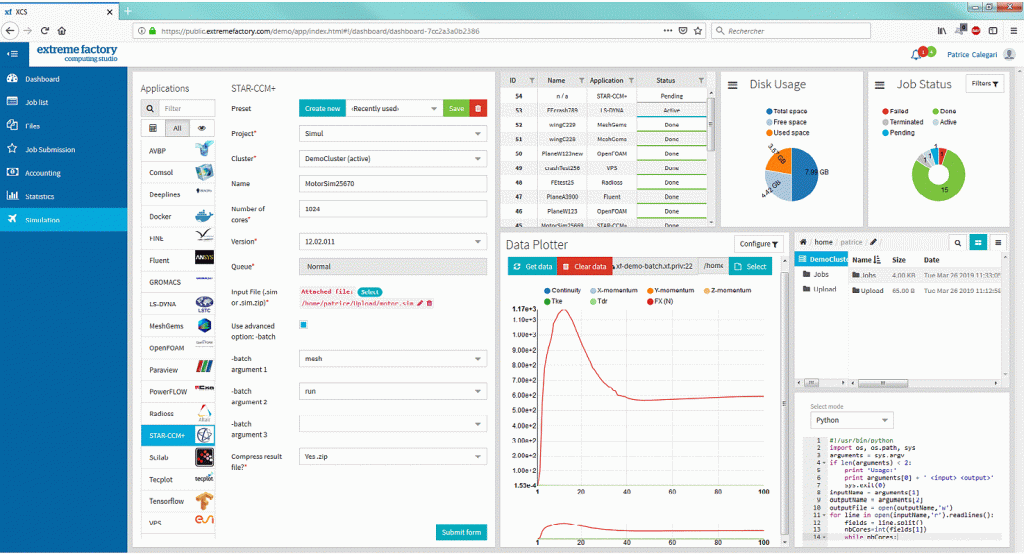
\includegraphics[width=1\textwidth]{Figures/atos-dashboard.png}
	\caption{Snímek aplikace The Smart HPC Web Portal \cite{l9RorNxGDyQGAn8I}}
	\label{fig:atos-dashboard}
\end{figure}

\newpage
Vizualizace a následné zpracovávání výsledků je možné prostřednictvím modulu, který je součástí zmiňovaného správcovského rozhraní. Výsledky lze zpracovávat vzdáleně přímo na serveru a na pracovní stanici uživatele se šifrovaně přenášejí pouze zkomprimovaná data (obrázky) \cite{y148btMogHCsnpoe}. Příklad takové vizualizace v rozhraní popisovaného modulu se nachází na obrázku \ref{fig:atos-3d}.


\begin{figure}[!h]
	\centering
	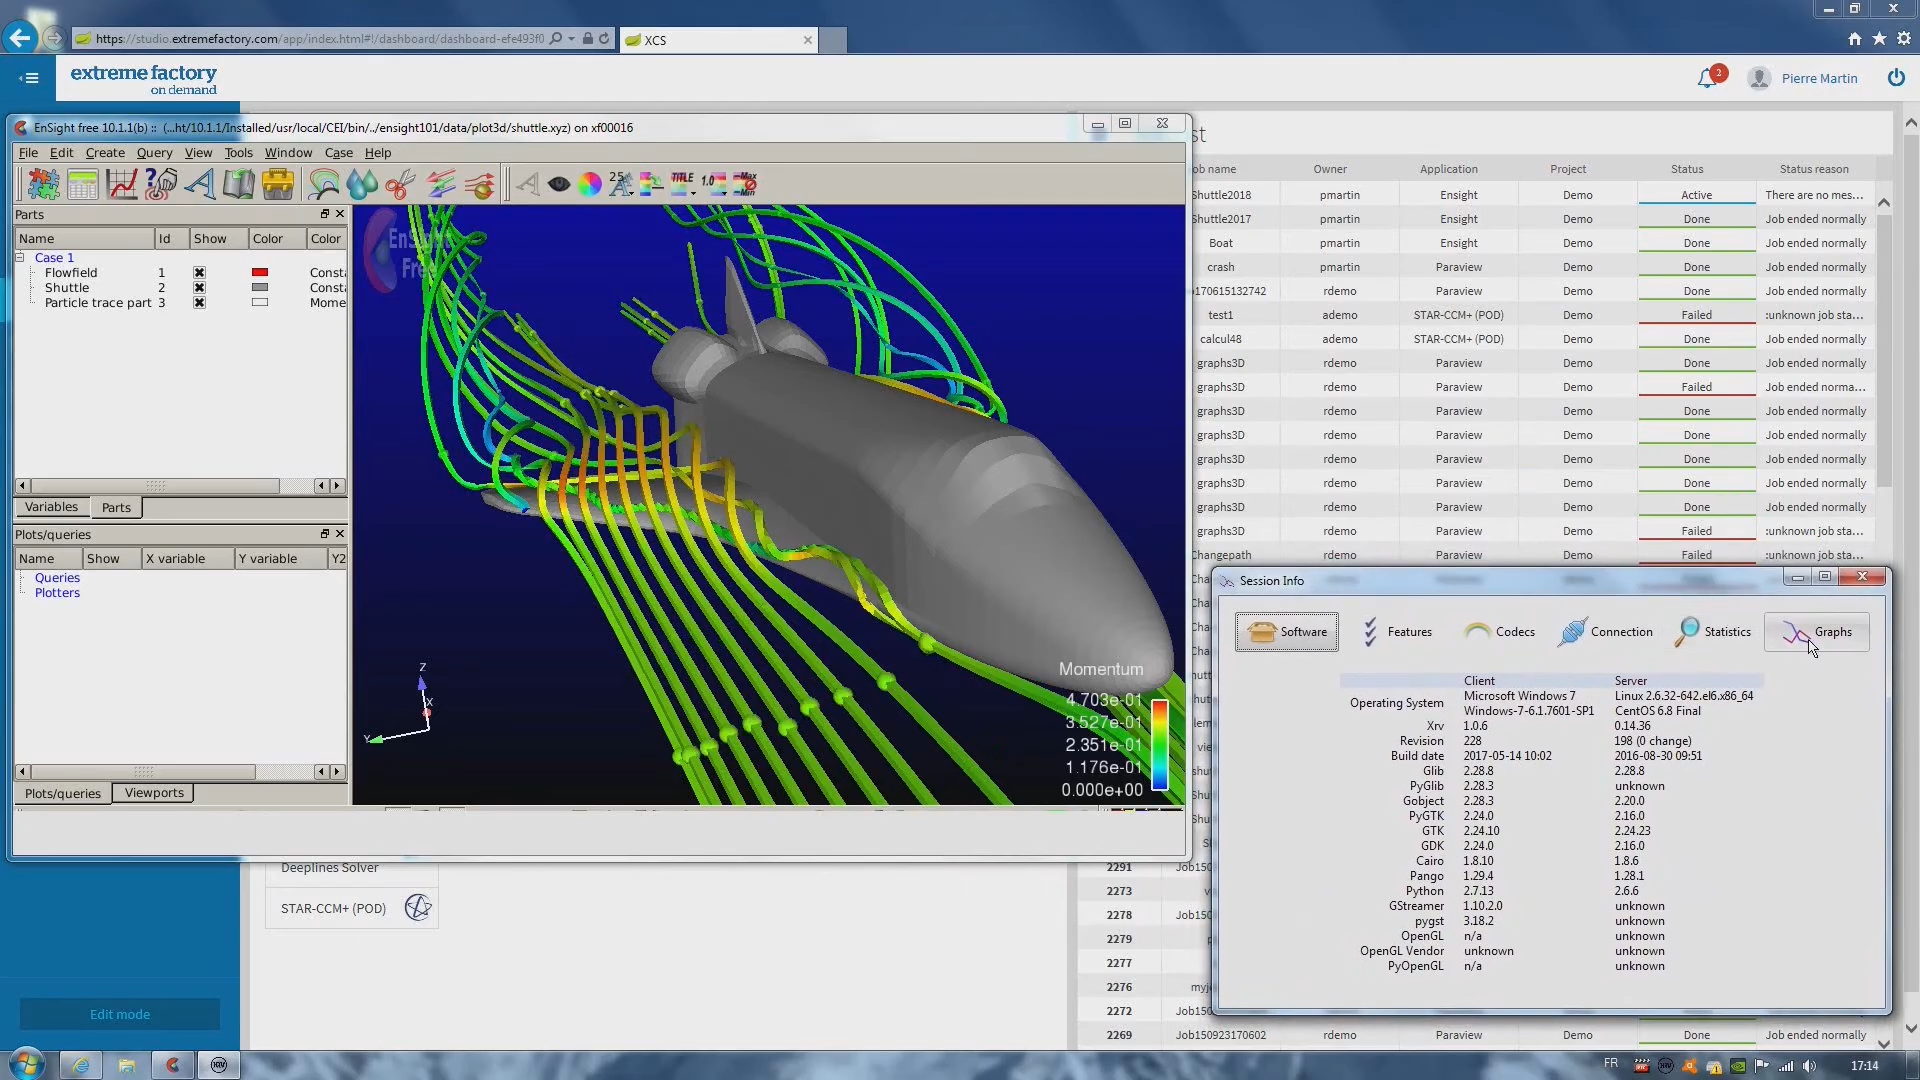
\includegraphics[width=1\textwidth]{Figures/bull-extreme-factory.png}
	\caption{Snímek aplikace Atos Extreme Factory \cite{l9RorNxGDyQGAn8I}}
	\label{fig:atos-3d}
\end{figure}